\documentclass{fizraport}
\authorA{Krzysztof Stasiowski}
\authorB{Joanna Binek}
\team{2}{2a}{1}

\topic{Opracowanie danych pomiarowych}{0}
\carryOutDate{03.10.2018 r.}
\ftHandInDate{10.10.2018 r.}

\begin{document}

\maketitle

\section{Cel ćwiczenia}
Zaznajomienie się z typowymi metodami opracowania danych pomiarowych
przy wykorzystaniu wyników pomiarów dla wahadła prostego.

\section{Wstęp}
Wahadło proste jest, jak wskazuje jego nazwa, układem mechanicznym charakteryzującym się prostotą tak  eksperymentu  jak  i  opisu  teoretycznego.
Dlatego nadaje  się dobrze  na ćwiczenie  wprowadzające (zerowe),   mające   na   celu   poznanie   podstawowych   metod   opracowania danych   pomiarowych.
Interpretacja  wyników  opiera  się na  równaniu  określającym  okres  drgań $T$ jako  funkcję długości wahadła $l$ oraz przyspieszenia ziemskiego $g$, 
%
\[ T = 2\pi \sqrt{\frac{l}{g}} \]
%
Wzór ten jest słuszny, jeżeli wychylenie ciężarka z położenia równowagi jest małe.  
Przekształcając powyższy wzór możemy wyznaczyć wartość przyspieszenia ziemskiego:
%
\[ g = \frac{\pi^2l}{T^2} \]

Zgodnie z powyższym opisem poniższe sprawozdanie skupia się na poznaniu metod,
mających na celu poprawną interpretację danych zdobytych podczas wykonywania następnych ćwiczeń.

\section{Opis Doświadczenia}

\begin{wrapfigure}{r}{0.34\textwidth}
 \centering
 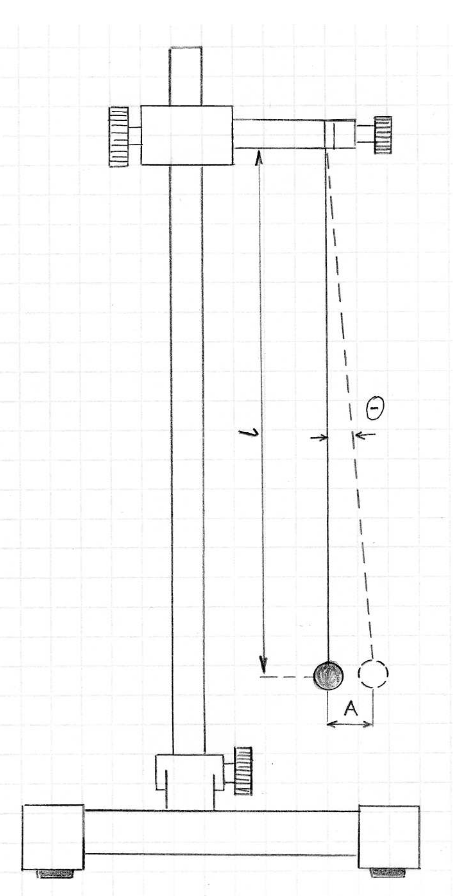
\includegraphics[width=0.27\textwidth,keepaspectratio=true]{wahadlo1.png}
 % wahadlo1.png: 474x896 px, 72dpi, 16.72x31.60 cm, bb=0 0 474 896
 \caption{Wachadło proste}
 \label{fig:w1}
\end{wrapfigure}

Zostały wykonane 2 rodzaje badań. Do obu zostało wykorzystane wahadło przedstawione na \figurename{\ref{fig:w1}}.

Składa się ono z~cylindrycznego mosiężnego odważnika zawieszonego na cienkiej lince. Linka została powieszona na wolnostojącym statywie - umożliwiającym regulację długości linki.
Pomiary były dokonywane za pomocą stopera o~dokładności~0.01s. Do niepewności pomiaru stopera należy dodać czas reakcji osoby wykonującej pomiary, który został ustalony na 0.1s.

Długość wahadła została zmierzona za pomocą linijki o~podziałce~1mm, niestety dokładność wyznaczenia długości jest mniejsza z~powodu konieczności oszacowanie środka częstości cylindra i~została określona~na~5mm.


\subsection{Pomiary przy stałej długości linki}
Pierwszymi wykonanymi pomiarami była seria pomiarów okresu~($T$). Zmierzyliśmy długość linki i~otrzymaliśmy wynik ??cm. 

Wychyliliśmy wahadło o~niewielki kąt z~położenia równowagi i~puściliśmy . Następnie zmierzyliśmy przy pomocy stopera 20~pełnych okresów wahadła. Czynności te~powtórzyliśmy 15 razy i~uzyskaliśmy wyniki podane w~\tablename{\ref{tab:e1}}. 

\subsection{Pomiary przy różnej długości linki}
Drugimi wykonanymi pomiarami była seria pomiarów okresu, przy~zmieniającej się długości linki~($l$). 

Ponownie zmierzyliśmy długość wahadła,następnie wychyliliśmy wahadło o~niewielki kąt z~położenia równowagi i~puściliśmy .  Zmierzyliśmy przy pomocy stopera 20 pełnych okresów wahadła, a~potem zmieniliśmy długość wahadła. Czynności te~powtórzyliśmy 9 razy i~uzyskaliśmy wyniki podane~w~\tablename{\ref{tab:e2}}. 

\section{Opracowanie Wyników}
%%todo Asia stuff
\begin{table}
\caption{tabelu 1}
 \label{tab:e1}
\end{table}

\begin{table}
\caption{tabele 2}
 \label{tab:e2}
\end{table}
\section{Podsumowanie}


\end{document}


























